\documentclass[12pt]{article}
\usepackage[margin=1.0in]{geometry}
\usepackage{graphicx}
\bibliographystyle{plain}
\usepackage{mathtools}
\usepackage{subfigure}

\begin{document}

\section{Specific Aim 2.1}

SET domain protein models of SETD2 and NSD2 were built using Modeller with PDBs 4FMU and 3OOI as inputs, respectively.  Proteins were placed in TIP3P water boxes of approximately 7 nm, with NaCl ions added to achieve neutrality.  The ff99sb-ildn force field \cite{lindorff2010improved} was used.  Systems were held at constant temperature (300K) and pressure (1 atmosphere) using a Langevin integrator and Monte Carlo barostat, as implemented in OpenMM 6.0.1 \cite{openmm2012}.  For each system, a total of 50-100 $\mu s$ of simulations was analyzed using MDTraj \cite{mdtraj2014}, MSMBuilder \cite{beauchamp2011msmbuilder2}, and Mixtape.  Slow coordinates were selected using temporal independent component analysis (tICA) \cite{schwantes2013improvements, perez2013identification} with randomly selected geometric features as inputs.  Seven-state Markov state models were constructed by Gaussian mixture model clustering of the two slowest linear combinations of features.

\begin{figure}
\subfigure[]{
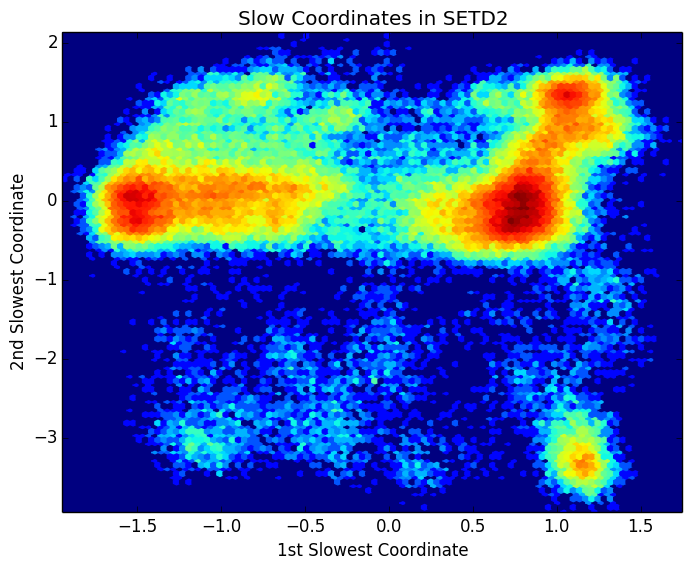
\includegraphics[width=7.0cm]{figures/SETD2_tics.png}
}
\subfigure[]{
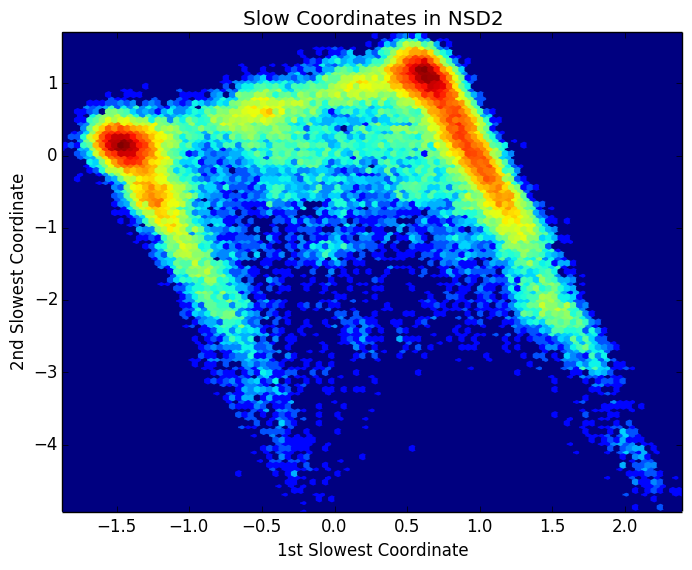
\includegraphics[width=7.0cm]{figures/NSD2_tics.png}
}


\subfigure[]{
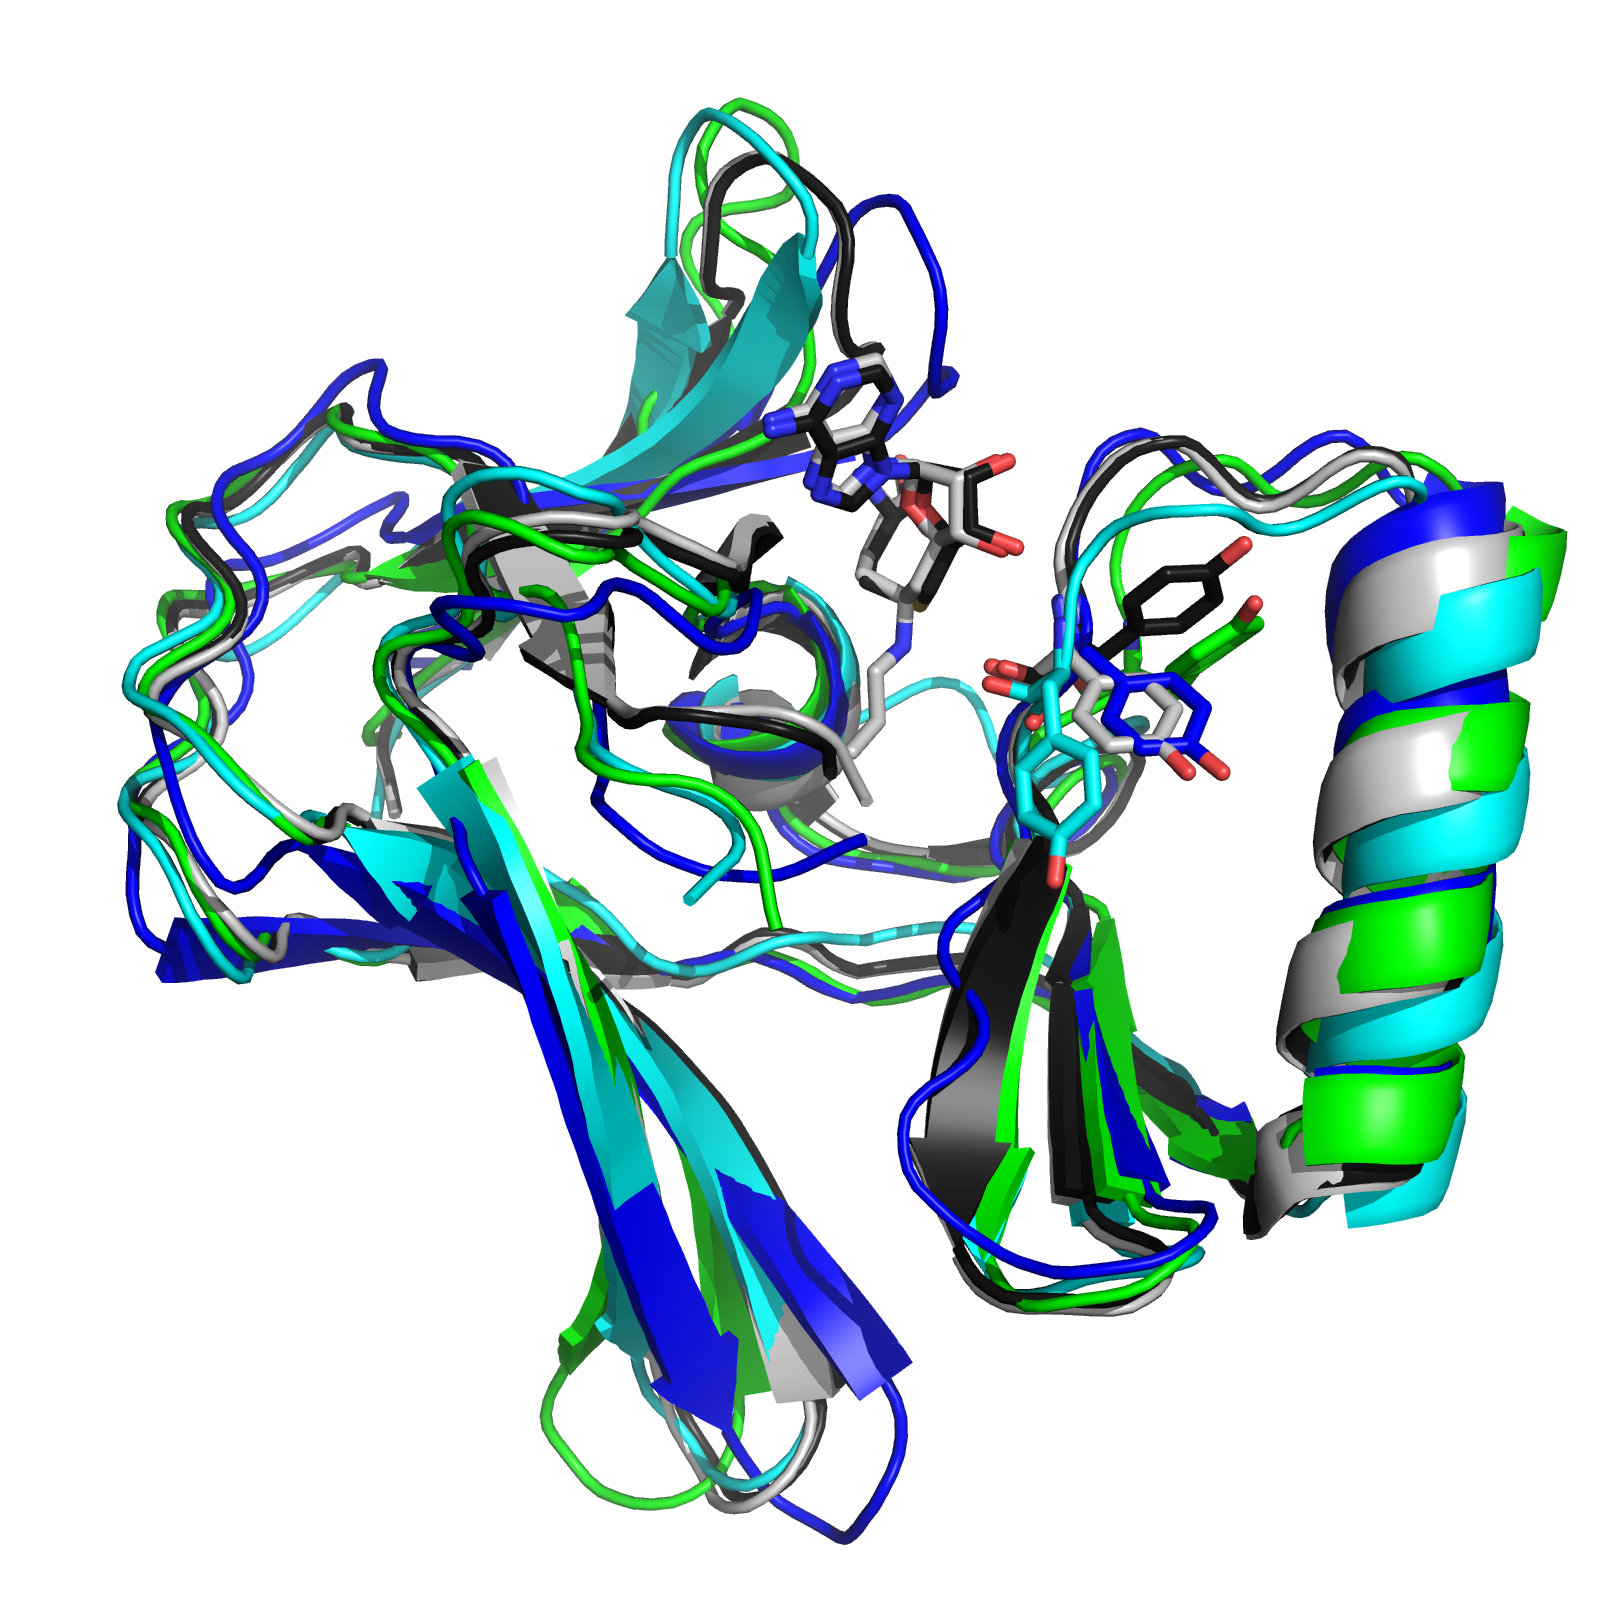
\includegraphics[width=7.0cm]{figures/SETD2_pdb.png}
}
\subfigure[]{
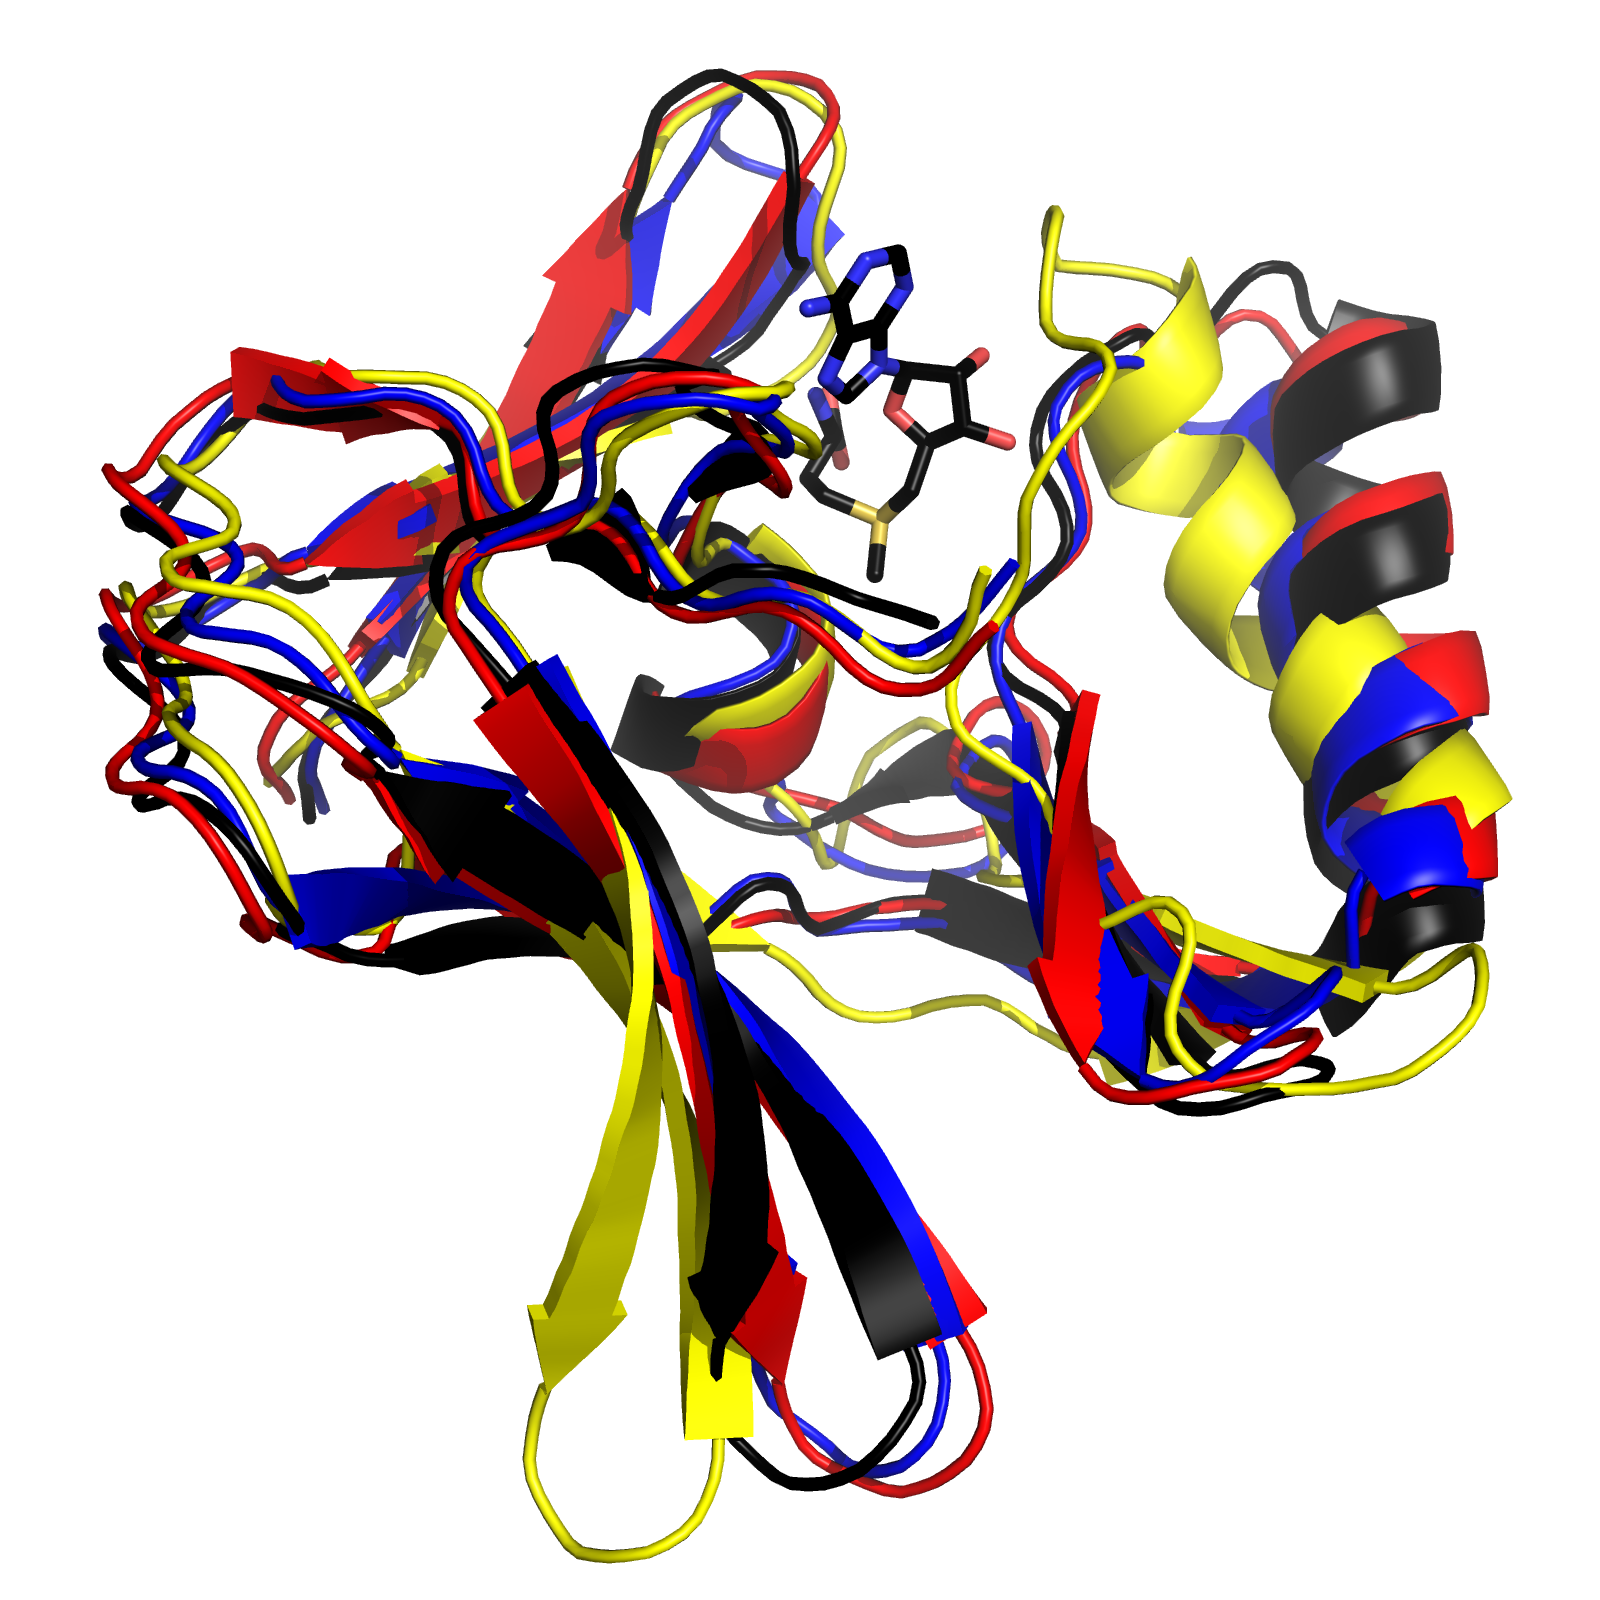
\includegraphics[width=7.0cm]{figures/NSD2_pdb.png}
}

\caption{
(a, b).  Conformational landscapes---projections onto the two slowest coordinates---show multiple heterogeneous conformational states observed in simulations at the $\approx 50 \mu s$ timescale.  (c, d). Structural comparisons indicate conformational heterogeneity near the known SAM / sinefungin binding site.  Ligand-bound crystal structures (gray, black) show similar conformational states.  (c).  SETD2 bound to SAH (black) adopts a TYR-up orientation (PDB:4H12), while SETD2 bound to sinefungin (gray) adopts a TYR-down orientation (PDB:4HMU); our simulation models (color) recapitulate the subtle conformational differences between these states.  (d).  Similar conformational heterogeneity is observed in models for NSD2 (color).  Because no crystal structure is available for NSD2, NSD1 (with SAM bound) is shown for comparison (black).  Simulations of SETD2 and NSD2 suggest that novel therapeutics might target and stabilize alternative near-native conformations, as has been observed in selective kinase inhibitors.
}
\label{figure:MSM}
\end{figure}


\bibliographystyle{plain}
\bibliography{TR01}

\end{document}
